
%Metadata architecture
\begin{frame}{Proposed cosmic-ray metadata structure}
    \vspace{-1.5em}
    \begin{center}
        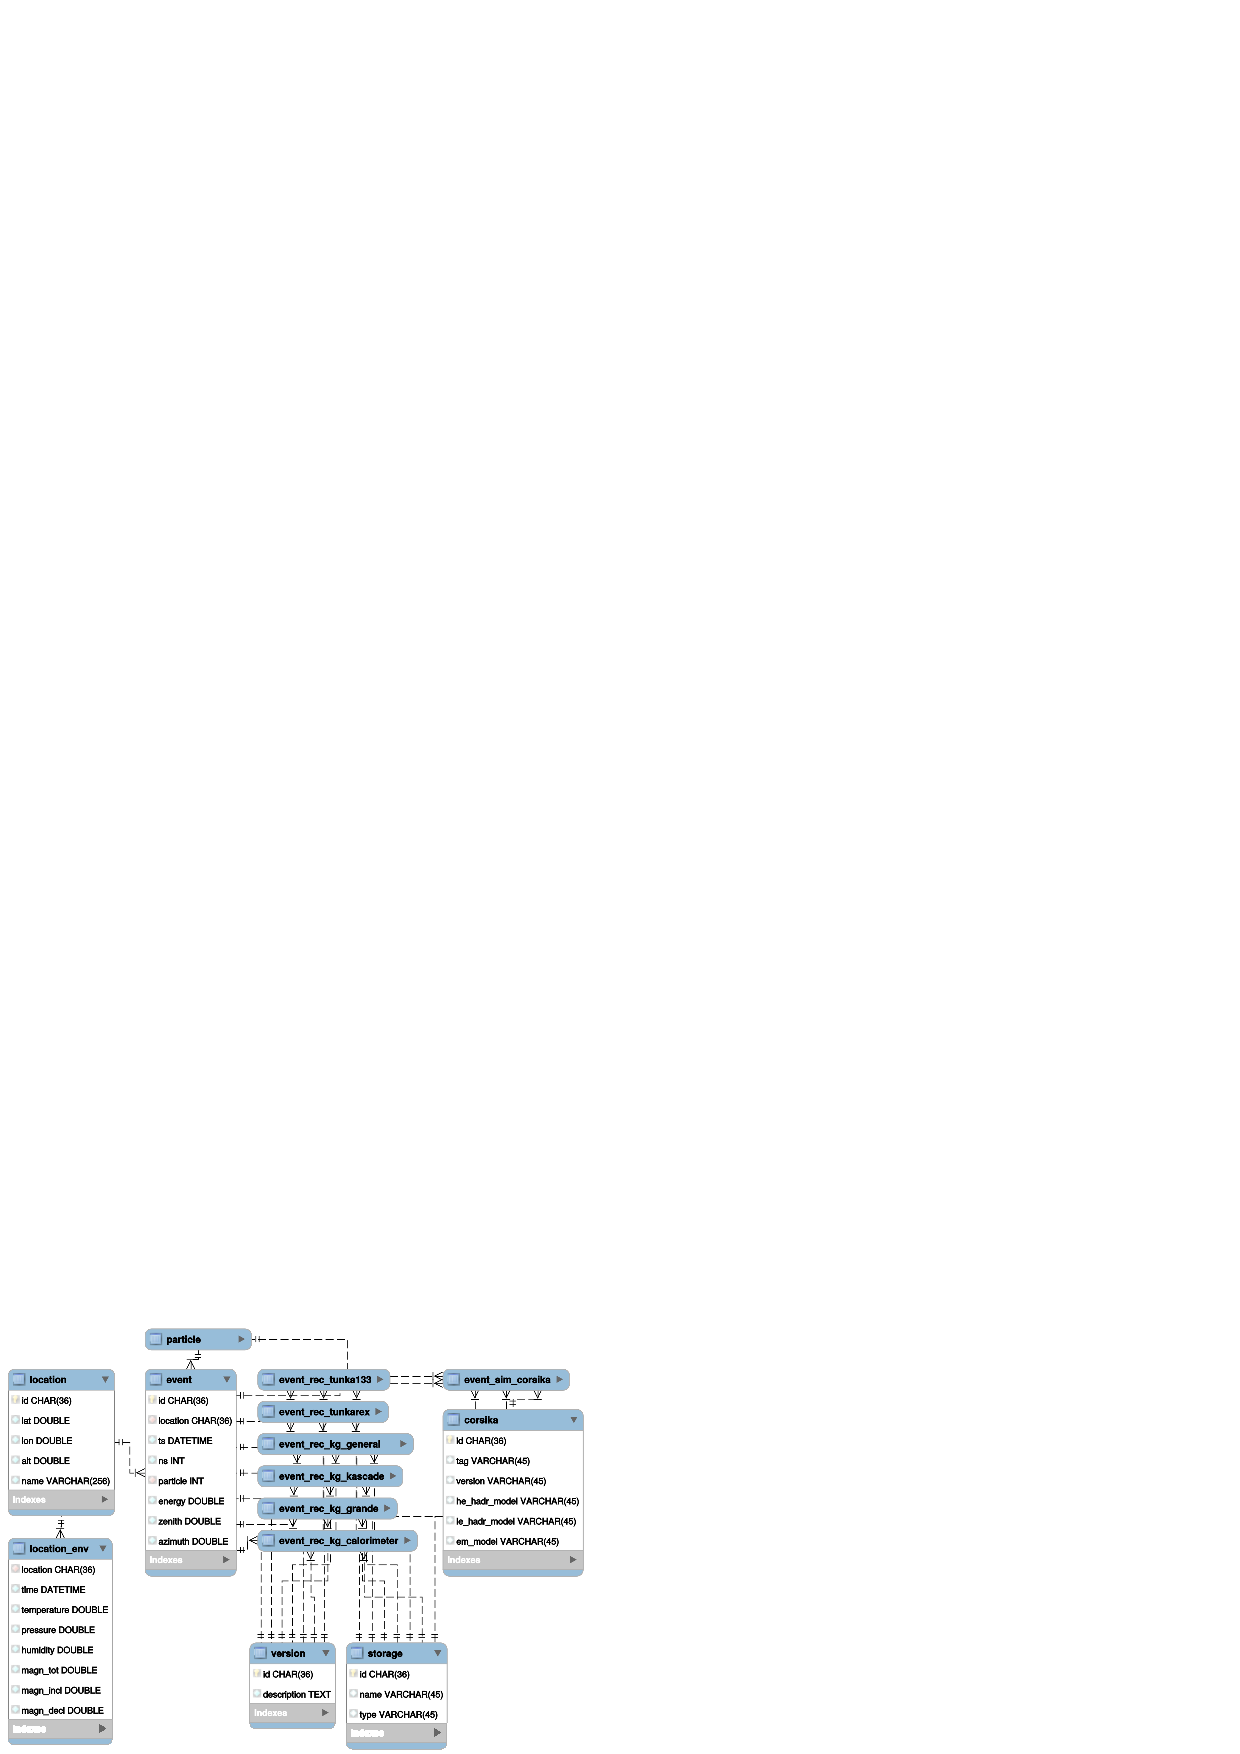
\includegraphics[width=0.82\textwidth]{pics/metadata.pdf}
    \end{center}
\end{frame}

% Data aggregation server:
\begin{frame}{Requirements for the data storage}
  \begin{itemize}
    \item Multiple experiments (TAIGA, KASCADE, etc.);
    \item Terabytes of data (of different reconstruction level) at each site;
    \item Remote access to query results as local file systems;
    \item  On-demand data transfer by requests only;
    \item  Automatic real-time updates;
    \item  No changes to existing site infrastructure, only add-ons.
  \end{itemize}
  \vspace{1em}
  \textbf{Main solution components}: CVMFS, PostgreSQL, TPL.
\end{frame}
